
\cleardoublepage\phantomsection
\pagepart
        {ANNEXES}
        {part_an}
        {ANNEXES : Chapitre}
        {ANNEXES : }
        {}
        
%\extraPartText{ }

% \part*{\linia
%         \bigskip
%         ANNEXES
%         \bigskip
%         \linia}
% 
% \addtocontents{toc}{\protect\vspace{2ex}\textbf{ANNEXES }\par}     
% \refstepcounter{part}\label{part_an}
% \renewcommand{\chaptername}{ANNEXES : Chapitre}
% \renewcommand\Partie{ANNEXES : }
\setcounter{chapter}{0}

\annexe{Explication mathématique et interprétation des termes des lois KHM}{an:A}\chapter{Explication mathématique et interprétation des termes des lois \acs{KHM}}
\renewcommand\partie{\Partie\ Chapitre \thechapter}
\label{an:A}

En s'inspirant de la démonstration mathématique de la convergence des fonctions de structures d'ordres 2 proposée par [\cite{cho_simulations_2009}], j'ai démontré le comportement des termes du type fonction de corrélation en fonction des tendances des spectres des quantités impliquées. La démonstration proposée ici est un résumé. 

Soit $A$ et $B$ deux quantités quelconques dépendant de $\mathbf{x}$.
Soit $a_{\boldsymbol{k}}$ (resp. $b_{\boldsymbol{k}}$) la transformée de Fourier de $A$ (resp. $B$) évaluée en  $\boldsymbol{k}$. Pour faciliter la lecture, on supposera les moyennes effectuées sur un volume $V$ = 1 et les intégrales triples ne seront notées qu'avec un seul $\int$. Dans cette Annexe, $\delta$ est la distribution de Dirac. 

La fonction de corrélation $\left<A\left({\bf x} + \boldsymbol{\ell}\right)  \cdot B\left({\bf x}\right)\right>$ est d'abord explicitée sous forme d'intégrale. Puis, les transformées de Fourier de $A$ et $B$ sont injectées. Quelques manipulations des différentes intégrales  sont nécessaires pour faire apparaître $\delta\left(\boldsymbol{k+k'}\right)$ qui nous permet de remplacer $\boldsymbol{k'}$ par $-\boldsymbol{k}$ : 
\begin{eqnarray}
\left<A\left({\bf x} + \boldsymbol{\ell}\right)  \cdot B\left({\bf x}\right)\right> &=& \int A\left({\bf x} + \boldsymbol{\ell}\right) \cdot B\left({\bf x}\right) d{\bf x} \\
&=& \int \left(\int a_{\boldsymbol{k}} e^{i\boldsymbol{k}\cdot\boldsymbol{x}} e^{i\boldsymbol{k}\cdot\boldsymbol{\ell}} d{\bf k} \right)\left(\int b_{\boldsymbol{k'}} e^{i\boldsymbol{k'}\cdot\boldsymbol{x}} d{\bf k'}\right) d{\bf x}  \\ 
&=& \int \int a_{\boldsymbol{k}}  e^{i\boldsymbol{k}\cdot\boldsymbol{\ell}}  b_{\boldsymbol{k'}}  \left(\int e^{i\left(\boldsymbol{k+k'}\right)\cdot\boldsymbol{x}}d{\bf x}\right)d{\bf k}d{\bf k'} \\
&\propto& \int \int a_{\boldsymbol{k}} b_{\boldsymbol{k'}} e^{i\boldsymbol{k}\cdot\boldsymbol{\ell}}    \delta\left(\boldsymbol{k+k'}\right) d{\bf k}d{\bf k'}\propto \int a_{\boldsymbol{k}}  b^*_{\boldsymbol{k}} e^{i\boldsymbol{k}\cdot\boldsymbol{\ell}}  d{\bf k} .\quad
\end{eqnarray}
Ensuite, la fonction de corrélation symétrique, $\mathcal{R}$, est construite en notant $\Re[Z]$ la partie réelle de $Z$, : 
\begin{eqnarray}
\mathcal{R} &=& \left<A\left({\bf x} + \boldsymbol{\ell}\right)  \cdot B\left({\bf x}\right) + A\left({\bf x}\right)  \cdot B\left({\bf x} + \boldsymbol{\ell}\right)\right> \\
&\propto& \int \left(a_{\boldsymbol{k}}  b^*_{\boldsymbol{k}} + a^*_{\boldsymbol{k}}  b_{\boldsymbol{k}}\right) \left(e^{i\boldsymbol{k}\cdot\boldsymbol{\ell}} + e^{-i\boldsymbol{k}\cdot\boldsymbol{\ell}}\right)  d{\bf k} \propto \int \Re[a_{\boldsymbol{k}}  b^*_{\boldsymbol{k}}] \cos\left(\boldsymbol{k}\cdot\boldsymbol{\ell}\right) d{\bf k}.
\end{eqnarray}

Pour une fonction de corrélation incrémentale, notée $\mathcal{S}$, l'expression finale sera un petit peu différente :
\begin{eqnarray}
\mathcal{S} &=& \left<\left(A\left({\bf x} + \boldsymbol{\ell}\right) - A\left({\bf x}\right)\right)\cdot\left(B\left({\bf x} + \boldsymbol{\ell}\right) - B\left({\bf x}\right)\right) \right> \\
&=& \left<2A\left({\bf x}\right)\cdot B\left({\bf x}\right) -  \left(A\left({\bf x} + \boldsymbol{\ell}\right)  \cdot B\left({\bf x}\right) + A\left({\bf x}\right)  \cdot B\left({\bf x} + \boldsymbol{\ell}\right)\right) \right>\\
&\propto& \int \left(a_{\boldsymbol{k}}  b^*_{\boldsymbol{k}} + a^*_{\boldsymbol{k}}  b_{\boldsymbol{k}}\right) \left(1 - e^{i\boldsymbol{k}\cdot\boldsymbol{\ell}} + e^{-i\boldsymbol{k}\cdot\boldsymbol{\ell}}\right)  d{\bf k} \propto \int \Re[a_{\boldsymbol{k}}  b^*_{\boldsymbol{k}}] \left(1-\cos\left(\boldsymbol{k}\cdot\boldsymbol{\ell}\right)\right) d{\bf k} .\qquad
\end{eqnarray}

Maintenant, nous allons explorer la convergence de ces intégrales pour quelques formes de spectres de $A$ et $B$ rappelant les comportements fréquentiels des termes de forçage et de dissipation.  

\section{Si $A$ correspond à une distribution de Dirac dans l'espace de Fourier} \label{an:forc} 

On suppose $a \propto \delta\left(\boldsymbol{k} - \boldsymbol{k_n}\right)$. Ce cas correspond au comportement du forçage utilisé dans la Partie \ref{part_3}. Dans ce cas :
\begin{eqnarray}
\mathcal{R} = <A\left({\bf x} + \boldsymbol{\ell}\right)  \cdot B\left({\bf x}\right) + A\left({\bf x}\right)  \cdot B\left({\bf x} + \boldsymbol{\ell}\right)> 
&\propto& \Re[b_{\boldsymbol{k_n}}] \cos\left(\boldsymbol{k_n}\cdot\boldsymbol{\ell}\right), \\
\mathcal{S} = <\left(A\left({\bf x} + \boldsymbol{\ell}\right) - A\left({\bf x}\right)\right)\cdot\left(B\left({\bf x} + \boldsymbol{\ell}\right) - B\left({\bf x}\right)\right) > 
&\propto&\Re[b_{\boldsymbol{k_n}}] \left(1-\cos\left(\boldsymbol{k_n}\cdot\boldsymbol{\ell}\right)\right) .\nonumber \\
\end{eqnarray}

Aux petites échelles telles que $\boldsymbol{\ell} \ll 1/\boldsymbol{k_n}$ et en représentation logarithmique, $\mathcal{R}$ sera donc constant puisque $ \cos\left(\boldsymbol{k_n}\cdot\boldsymbol{\ell}\right)\sim 1 $ et que $ \Re[b_{\boldsymbol{k_n}}]$ est indépendant de $\boldsymbol{\ell}$. On retrouve le comportement de $\varepsilon_{F}$ (voir \ref{ch-32}). Pour ce qui est de $\mathcal{S}$, $ \left(1-\cos\left(\boldsymbol{k_n}\cdot\boldsymbol{\ell}\right)\right) \sim \left(\boldsymbol{k_n}\cdot\boldsymbol{\ell}\right)^2$ et on retrouve la pente de facteur $2$  observée pour $\mathcal{E}_{F}$ en représentation logarithmique. 

\section{Si \ensuremath{\Re[a_{\boldsymbol{k}}  b^*_{\boldsymbol{k}}]} est proportionnelle à une puissance de l'amplitude de $\boldsymbol{k}$ } \label{an:sat}

On suppose l'hypothèse d'isotropie pour simplifier le calcul\footnote{Dans le cas axisymétrique, il faut gérer les directions parallèle et perpendiculaire. Le calcul se complique, mais les tendances resteront similaires.} et on explicite les quantités vectorielles dans un système de coordonnées sphérique,  $\{k,\phi,\theta\}$, orienté tel que $\theta$ soit l'angle entre $\boldsymbol{k}$ et $\boldsymbol{\ell}$. Alors $d{\bf k} = k^2 \sin \theta dk d\theta d\phi$ avec $\theta \in [0,\pi]$ et $\phi \in [0,2\pi]$, et $\boldsymbol{k}\cdot\boldsymbol{\ell} = k\ell \cos\theta$. 

On note aussi $k^{2} \Re[a_{\boldsymbol{k}}  b^*_{\boldsymbol{k}}] \propto k^{-m}$. Ce cas est le plus commun dans les études de turbulence. En effet, par exemple, la phénoménologie de Kolmogorov indique un spectre d'énergie cinétique,  $k^2 \boldsymbol{v}^2_k$, proportionnel à $k^{-5/3}$. Pour ce qui est de l'hyperdissipation $\Delta^4 \sim k^8$. Dans [\cite{ferrand_multi-scale_2021}], est indiqué pour l'hyperdissipation cinétique incompressible, un spectre en $k^8 \boldsymbol{v}^2_k \sim k^6$ . Dans le cas compressible, on supposera que les spectres liés à l'hyperdissipation ont une pente telle que $m \ll -1$.

Avec ces hypothèses, on obtient :
\begin{eqnarray}
\mathcal{R} \propto \int_k \int^{\pi}_0 k^{-m} \cos\left(k\ell \cos\theta\right) \sin\left(\theta\right)dk d\theta &\propto& \int_k \int^{\pi}_0 k^{-m} \frac{\sin\left(k\ell\right)}{k\ell} dk \nonumber\\
\textrm{(par substitution $u = k\ell$) } &\propto& \ell^{m-1} \int_0^{+\infty} u^{-m-1} \sin\left(u\right) du ,\quad \\
\mathcal{S} \propto \int_k \int^{\pi}_0 k^{-m}  \left(1-\cos\left(k\ell \cos\theta\right)\right) \sin\left(\theta\right)dk d\theta &\propto& \ell^{m-1} \int_0^{+\infty} u^{-m} \left(1-\frac{\sin\left(u\right)}{u}\right) du .\nonumber \\
\end{eqnarray}

Ensuite, il est nécessaire de regarder la convergence de $K = \int_0^{+\infty} u^{-m-1} \sin\left(u\right) du$ afin d'estimer une tendance en $\ell$. Si $m \in ]-1,1[$, cette intégrale peut s'écrire comme une intégrale généralisée de Fresnel convergente et constante in $\ell$. Pour les deux autres ($]-\infty,-1[$ and $]1,+\infty[$), on peut obtenir une expression de récurrence en intégrant par partie $K$ puis estimer la convergence des différents termes. Alors, si $m \in ]-\infty,-1[$, $K\propto \ell^{-m-1}$ et si $m \in ]1,+\infty[$, $K\propto \ell^{-m+1}$. Par ces techniques, on obtient :
\begin{eqnarray}
    \mathcal{R} &=& <A\left({\bf x} + \boldsymbol{\ell}\right)  \cdot B\left({\bf x}\right) + A\left({\bf x}\right)  \cdot B\left({\bf x} + \boldsymbol{\ell}\right)> 
\propto \left\{
    \begin{split}
    &\ell^{-2}& \textrm{si $m \in ]-\infty,-1[$ } \\
 &\ell^{m-1}&  \textrm{si $m \in ]-1,1[$}  \\
 &1& \textrm{si $m \in ]1,+\infty[$ } 
\end{split}
\right.\nonumber  \\
&&\\
   \mathcal{S} &=& <\left(A\left({\bf x} + \boldsymbol{\ell}\right) - A\left({\bf x}\right)\right)\cdot\left(B\left({\bf x} + \boldsymbol{\ell}\right) - B\left({\bf x}\right)\right) > 
\propto \left\{
    \begin{split}
    & 1 & \textrm{si $m \in ]-\infty,1[$ } \\
& \ell^{m-1}&  \textrm{si $m \in ]1,3[$ }  \\
& \ell^2 & \textrm{si $m \in ]3,+\infty[$}
\end{split}
\right. \nonumber\\
\end{eqnarray}


Ces tendances sont représentées sur la figure \figref{fig:sat_corr} pour $\mathcal{R}$ et \figref{fig:sat_inc}. On retrouve aussi la prédiction de \cite{cho_simulations_2009} pour les fonctions de corrélation de type $\mathcal{S}$ avec $A=B$. Cette prédiction est étendue, ici, à $A\neq B$ et $m<0$. Passer de $\mathcal{R}$ à $\mathcal{S}$ est très simple : il suffit de soustraire à $\mathcal{R}$, sa valeur en $\ell = 0$ pour obtenir $\mathcal{S}$. L'équivalence est montrée sur la figure \figref{fig:sat_comp}. 

On s'attend donc à retrouver ce genre de saturations mathématiques dans nos simulations pour l'hyperdissipation qui se comporte tel que $m \ll -1$.

\begin{figure}
\center
     \begin{subfigure}[b]{0.496\textwidth}
         \centering
         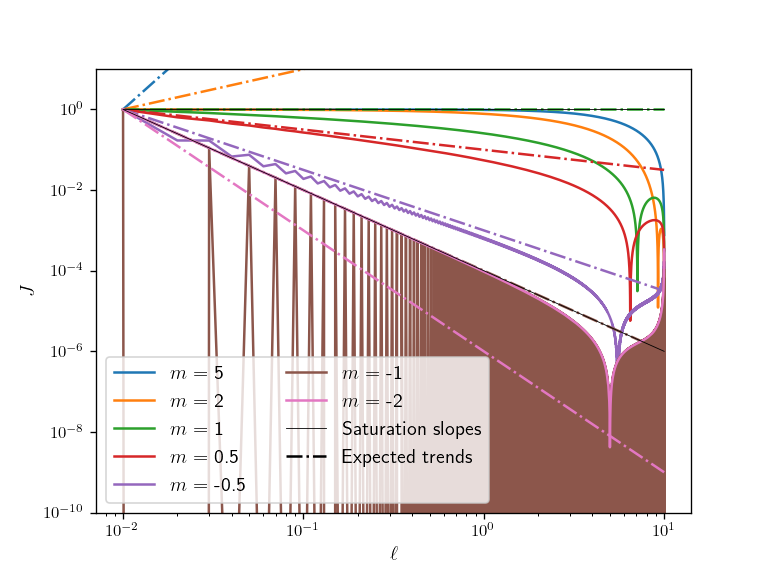
\includegraphics[width=\textwidth,trim = 0.5cm 0.5cm 2cm 2cm, clip]{./Part_Appendix/images/sat_cor}
         \caption{$\mathcal{R} = <A'\cdot B + A\cdot B'>$ }
         \label{fig:sat_corr}
     \end{subfigure}
     \hfill
     \begin{subfigure}[b]{0.496\textwidth}
         \centering
         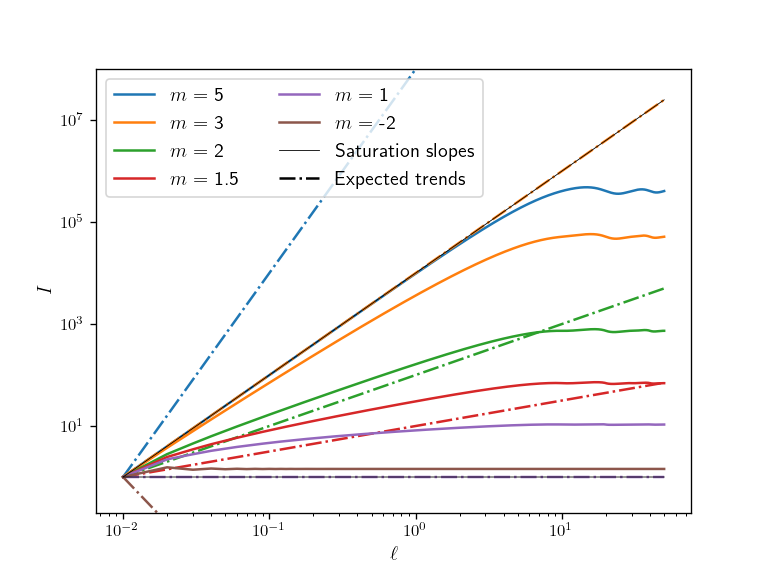
\includegraphics[width=\textwidth,trim = 0.5cm 0.5cm 2cm 2cm, clip]{./Part_Appendix/images/sat_inc}
         \caption{$\mathcal{S}=<\left(A'-A\right)\cdot\left(B'-B\right)>$ }
         \label{fig:sat_inc}
     \end{subfigure}
        \caption{Lignes pleines colorées : fonction de corrélation suivent la loi d'échelle spectrale de puissance $m$. Lignes discontinues colorées : tendance attendue pour chaque $m$ si n'y pas de saturation mathématique. Lignes fines noires : tendance des saturations. }
        \label{fig:sat_trends}
% \end{figure}
% \begin{figure}
% \center
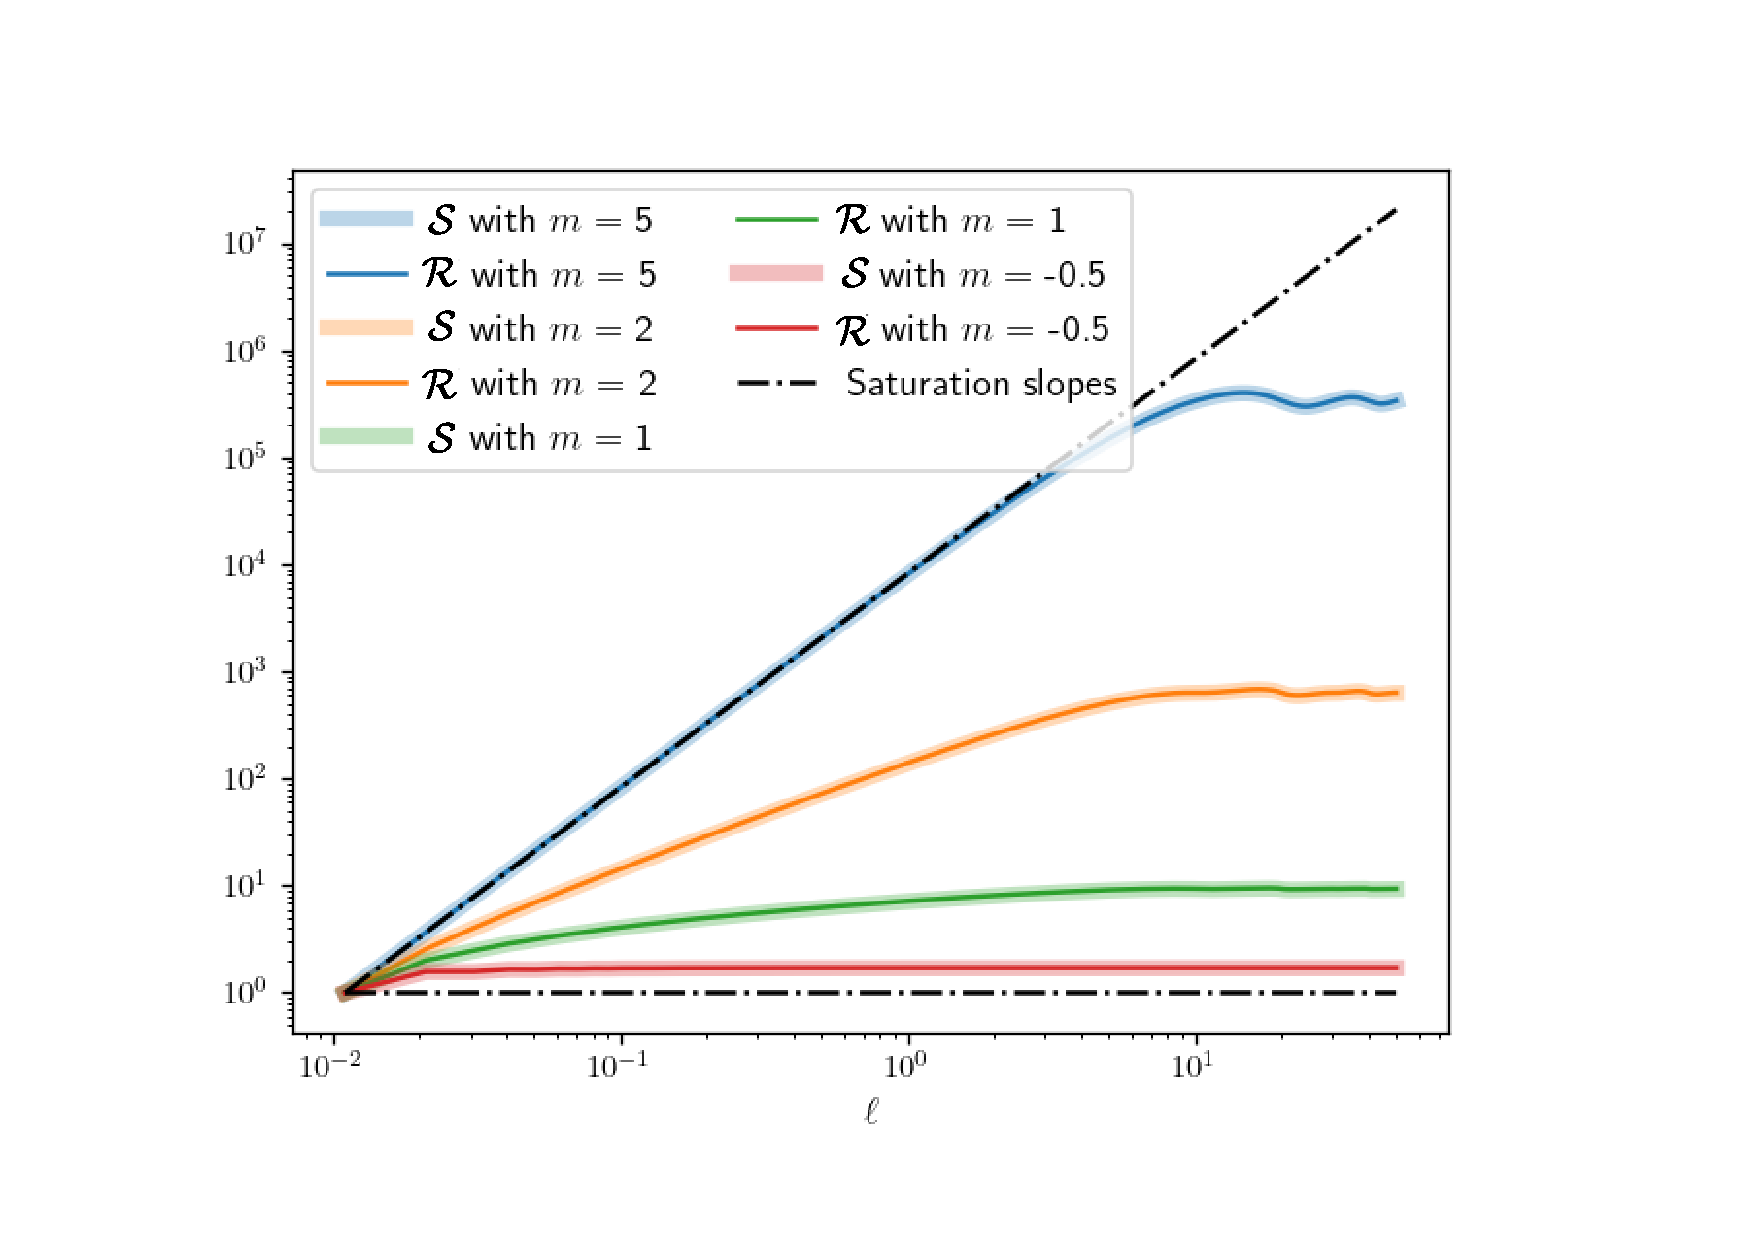
\includegraphics[width=0.5\textwidth,trim = 2cm 0.5cm 2cm 2cm, clip]{./Part_Appendix/images/sat_comp_2}
\caption{Équivalence entre $\mathcal{S}$ and $2<A\cdot B> - \mathcal{R}$. Couleurs : $m$. Lignes fines : $2<A\cdot B> - \mathcal{R}$. Lingnes épaisses: $\mathcal{S}$. Lignes discontinues : saturations. }
\label{fig:sat_comp}
\end{figure}


Cette démonstration montre que le lien entre tendance spectrale et fonction de corrélation n'est pas évident. Quelques pincettes sont donc à prendre lorsque l'on veut interpréter les résultats des lois \ac{KHM} en particulier à travers l'hypothèse de séparation d'échelle. Ce n'est pas parce que le forçage n'est supposé agir qu'à grande échelle que sa contribution, $\varepsilon_F$, à la loi \ac{KHM} tendra vers 0 aux autres échelles, elle va en effet rester constante. En fonction de sa forme, incrémentale ou non, la contribution dissipative sera ou constante ou de pente $2$ ou $-2$. \cite{ferrand_multi-scale_2021} a proposé quelques méthodes afin de contourner ce problème dans le cas incompressible mais leur validité est questionnable dans le cas compressible. Comme on a pu le remarquer, une méthode simple peut aider à l'interprétation de ces contributions : regarder conjointement les lois \ac{KHM} incrémentale ou non. Si les fonctions de corrélations permettant de les obtenir sont bien choisies, il est très facile de passer de l'une à l'autre en soustrayant les valeurs obtenues en $\ell=0$. 


\annexe{Validation et comparaison des lois exactes avec pression isotrope}{an:B}
 \section{Comparaison des formulations de la loi MHD incompressible} \label{an:compa_BG17}
 
  On propose ici une validation de notre code de post-traitement à travers une comparaison des formulations de la loi \cacro{PP98}.
  
 \begin{figure}[!ht]
  \centering
 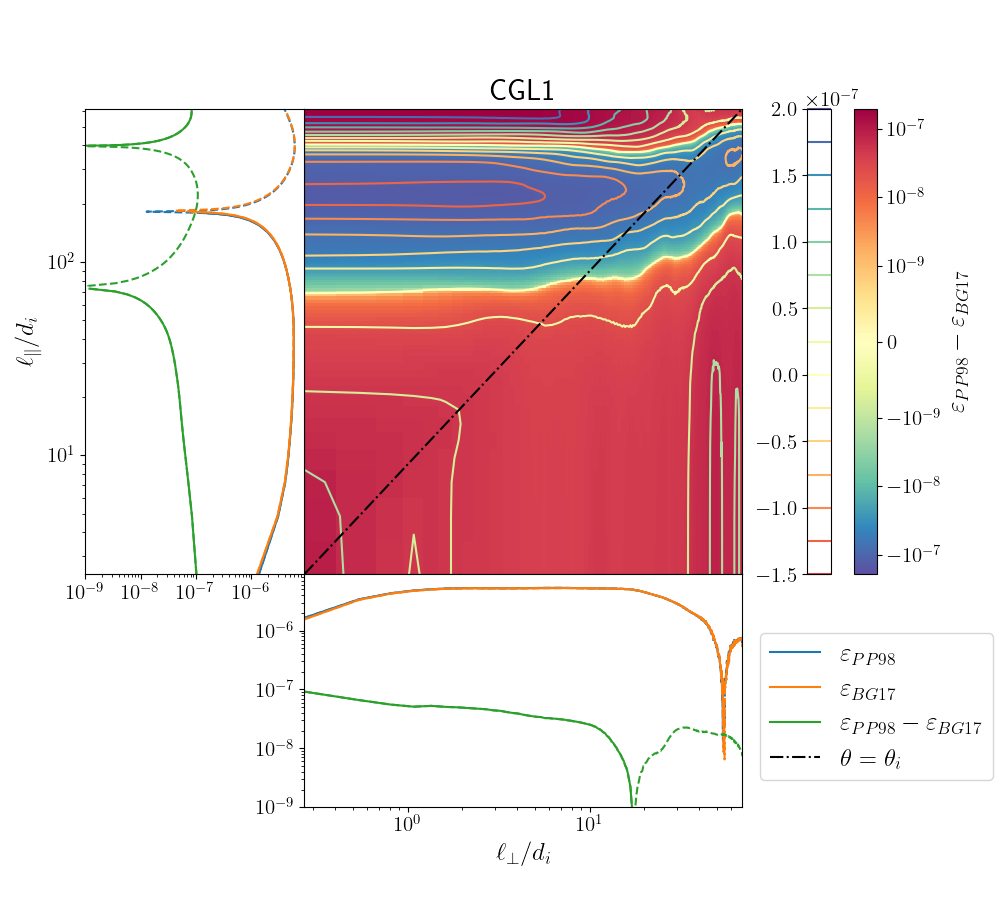
\includegraphics[width=0.75\linewidth,trim=0cm 1cm 0cm 2cm, clip=true]{./Mainmatter/Part_3/images_ch2/CGL1_BG17}
 %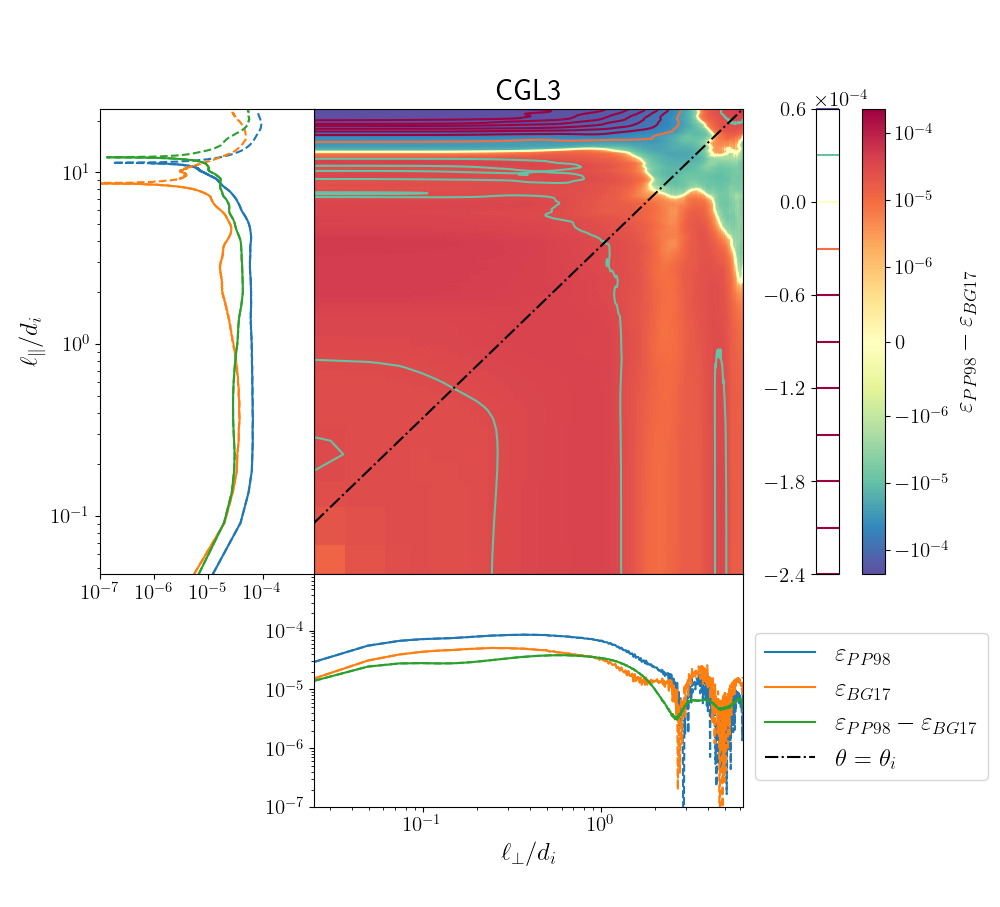
\includegraphics[width=0.8\linewidth,trim=0cm 1cm 0cm 1cm, clip=true]{./Part_3/images_ch2/CGL3_BG17}
 \cprotect\caption{Triptyques de la différence \ensuremath{\varepsilon_{PP98}-\varepsilon_{BG17}} (courbes vertes et carte 2D) calculée dans CGL1. Courbes 1D bleues : \ensuremath{\varepsilon_{PP98}}. Courbes 1D oranges : \ensuremath{\varepsilon_{BG17}} (coïncidant avec les bleues).}
 \label{fig:BG17}
  \end{figure}
  
 Elle peut en effet s'écrire via une autre formulation ne dépendant pas de $\nabla_{\boldsymbol{\ell}}$ mais dépendant de la vorticité $\boldsymbol{w} = \nabla \times \boldsymbol{v}$. Cette loi a été dérivée par \cite{banerjee_exact_2017}. Le taux de cascade associé sera noté $\varepsilon_{BG17}$, et s'écrit, sous un format non normalisé et avec nos notations, : 



\begin{equation}
     \varepsilon_{BG17} = \frac{1}{2} \left< \delta\left(\boldsymbol{v} \times \boldsymbol{w} + \sqrt{\mu_0} \boldsymbol{j} \times\boldsymbol{v_A}\right) \cdot \delta \boldsymbol{v} + \sqrt{\mu_0} \delta\left(\boldsymbol{v}\times \boldsymbol{v_A}\right)\cdot \delta \boldsymbol{j}\right> .
 \end{equation}
 
 Sur la  \figref{fig:BG17}, est représentée la différence $\varepsilon_{PP98}-\varepsilon_{BG17}$ suivant les différents modes de représentation retenus au Chapitre \ref{ch-31}. Cette figure nous indique que, quelle que soit l'échelle $\boldsymbol{\ell}$, $\varepsilon_{PP98}-\varepsilon_{BG17}$ est de l'ordre de $\num{e-7}$ maximum pour CGL1 et en moyenne de l'ordre de $\SI{2}{\%}$ du niveau moyen de $\varepsilon_{PP98}$ qui est de l'ordre de $\num{5e-6}$. On obtient ainsi une estimation relative de l'erreur effectuée sur $\varepsilon_{PP98}$. 
 
 Cette erreur pourrait provenir de la forme analytique de la dérivation, locale (BG17) à travers la vorticité  et la densité de courant ou en échelle (PP98) à travers la divergence en $\ell$, car elle n'est pas appliquée au même stade du schéma numérique ni avec les mêmes quantités. De plus, le passage analytique d'une forme à l'autre, n'est pas direct, la contrainte incompressible doit être utilisée. 
 
 \section{Résultats compressibles avec pression isotrope }
 \label{an:compa_predict}

 Ici, nous regardons avec CGL1, le comportement du taux de cascade compressible calculé en supposant une pression isotrope afin de comparer le résultat de la loi \eqref{eq:turb_elg_f1} aux comportements observés par \cacro{A18} dans le cas isotherme. 
 
 Dans la simulation CGL1, trois pressions sont disponibles, les pressions ioniques parallèle, $p_{\parallel i}$, et perpendiculaire, $p_{\perp i}$, et la pression électronique supposée isotherme, $p_{e} = \rho$. Nous calculerons la pression isotrope à partir de la formule $p = \frac{1}{3}\left(2p_{\perp i} + p_{\parallel i}\right) + p_{e}$ et l'énergie interne\footnote{ 
 L'énergie interne des ions est l'énergie interne gyrotrope : $\rho_i u_i = \frac{1}{2}\left(2p_{\perp i} + p_{\parallel i}\right)$. L'énergie interne des électrons s'obtient à partir du premier principe de la thermodynamique (cas isentrope-isotherme, voir Chapitre \ref{ch-12}) appliqué aux quantités électroniques et en supposant $p_e = \rho = \rho_i$ : $ u_e  = \frac{p_e}{\rho_e} \ln \left( \frac{\rho_e}{\rho_{e0}}\right) =   \frac{m_i}{m_e} \ln \left( \frac{\rho}{\rho_{0}}\right) $ avec $\rho_0 = 1$ (initialisation des simulations).} à partir de $\rho u = \frac{1}{2}\left(2p_{\perp i} + p_{\parallel i}\right) + \rho \ln \rho$.
 On s'attend à ce que le taux de cascade, noté $\varepsilon_{f_1}$, soit constant aux échelles MHD, la loi exacte étant obtenue dans le cadre d'une loi d'Ohm idéale valable si $\ell \gg d_i$. 

 \begin{figure}[!ht]
  \centering
 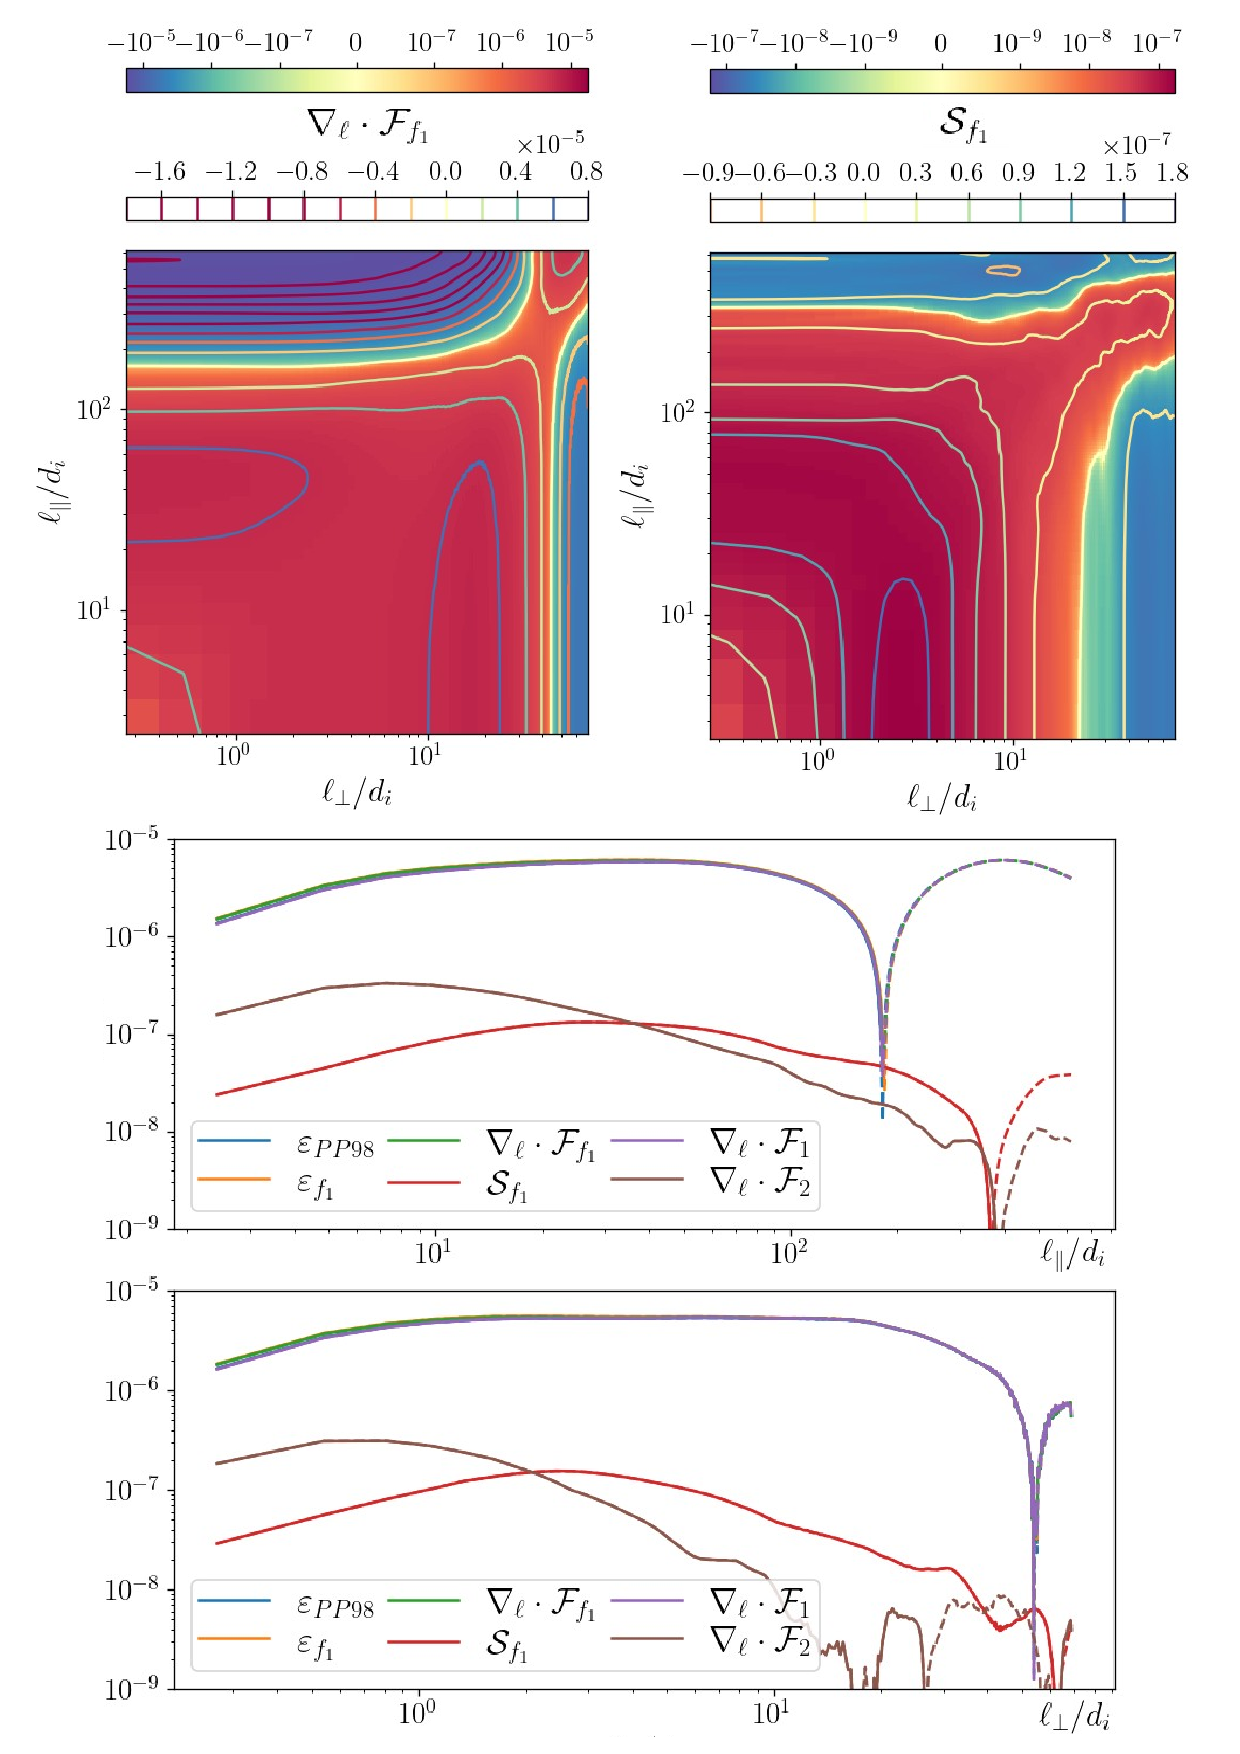
\includegraphics[width=0.8\linewidth,trim=0cm 0cm 0cm 0cm, clip=true]{./Mainmatter/Part_3/images_ch2/CGL1_f1}
 \cprotect\caption{Panel d'étude de \ensuremath{\varepsilon_{f_1}} dans CGL1. Première ligne de gauche à droite : Représentation 2D de \ensuremath{\nabla_{\boldsymbol{\ell}} \cdot \mathcal{F}_{f_1}}  et \ensuremath{\mathcal{S}_{f_1}}. Deuxième ligne : Représentation 1D en fonction de \ensuremath{\ell_{\perp}/d_i}. Troisième ligne : Représentation 1D en fonction de \ensuremath{\ell_{\parallel}/d_i}. Sur les représentations 1D : \ensuremath{\varepsilon_{PP98}} (bleu), \ensuremath{\varepsilon_{f_1}} (orange), \ensuremath{\nabla_{\boldsymbol{\ell}} \cdot \mathcal{F}_{f_1}} (vert), \ensuremath{\mathcal{S}_{f_1}} (rouge),  \ensuremath{\nabla_{\boldsymbol{\ell}} \cdot \mathcal{F}_1} (violet)  et \ensuremath{\nabla_{\boldsymbol{\ell}} \cdot \mathcal{F}_2} (marron).}
 \label{fig:elf1_CGL1}
 \end{figure}
% % \begin{figure}[!ht]
% %  \centering
% % 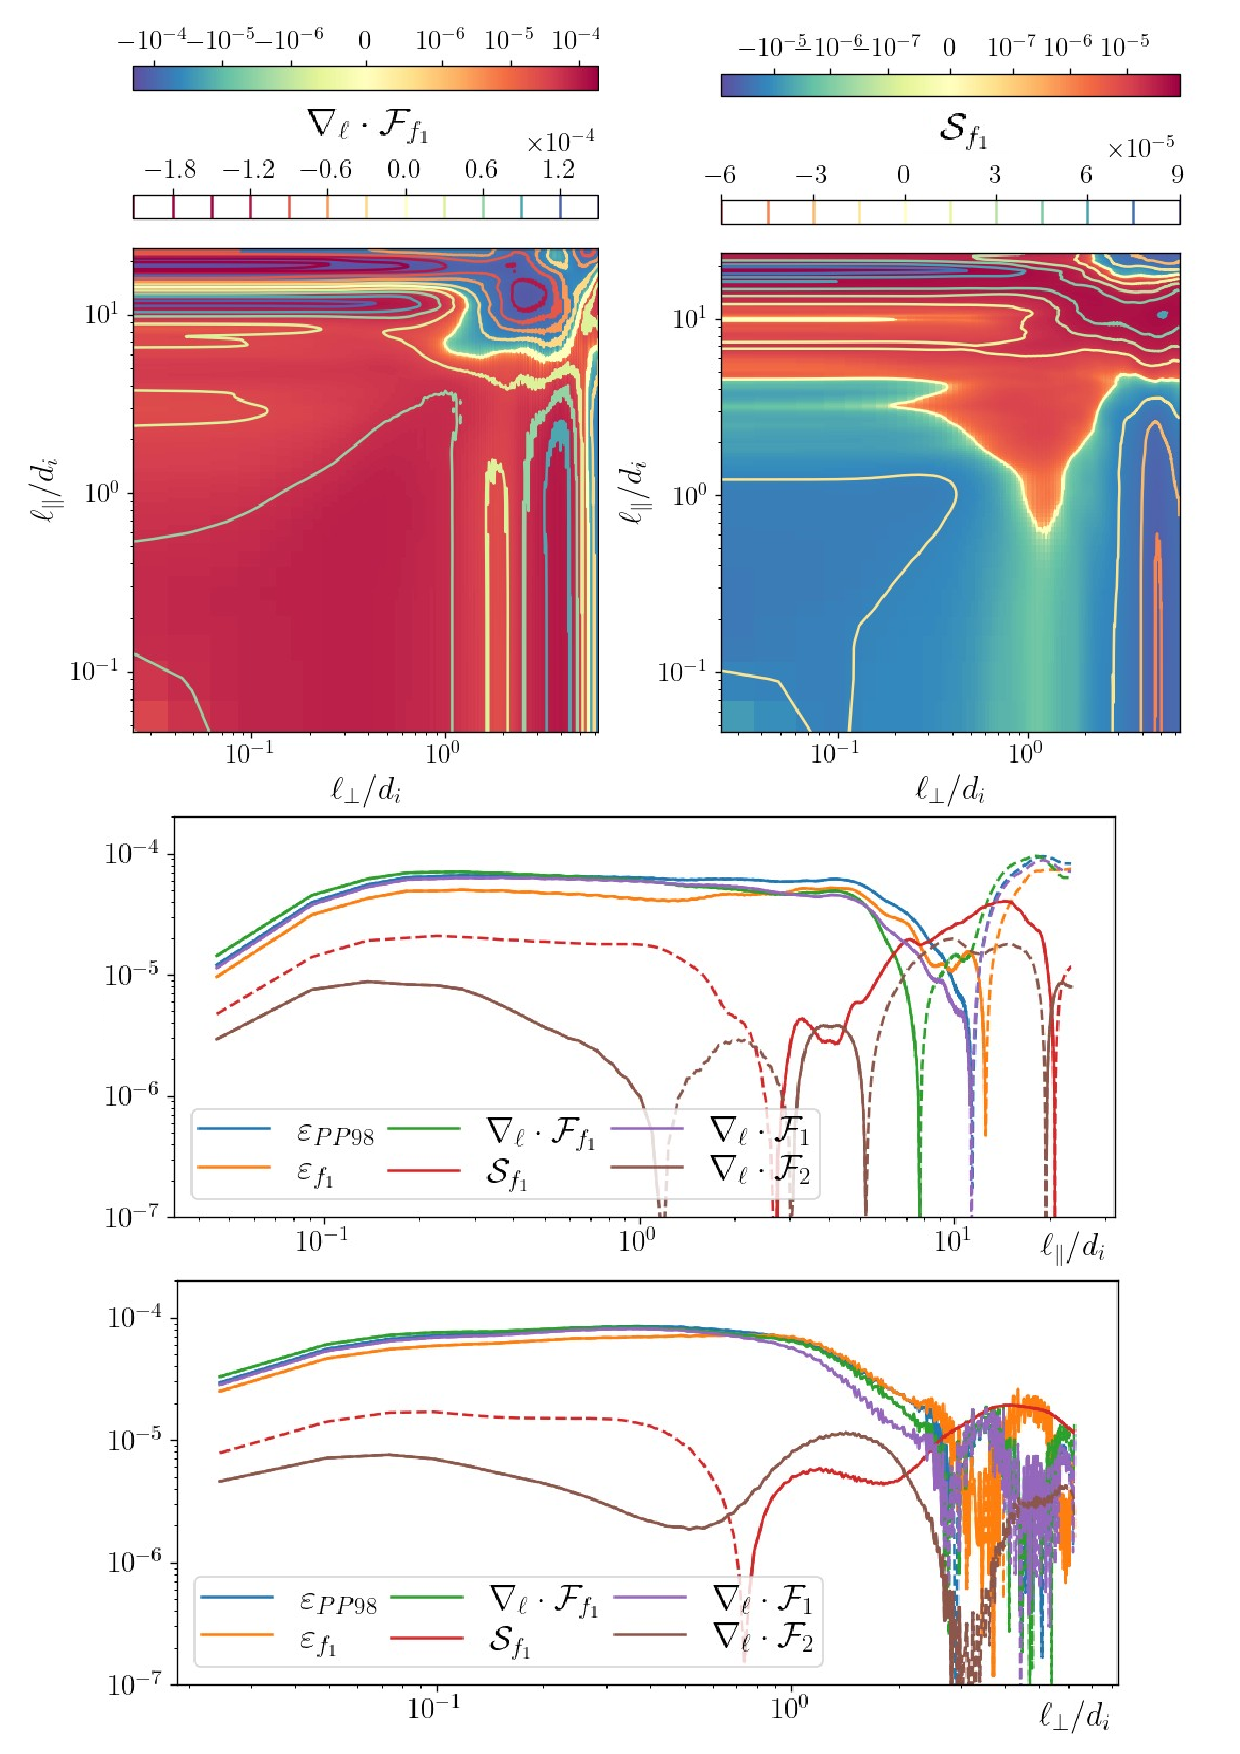
\includegraphics[width=0.9\linewidth,trim=0cm 0cm 0cm 0cm, clip=true]{./Part_3/images_ch2/CGL3_f1}
% % \cprotect\caption{Panel d'étude de $\varepsilon_{f_1}$ dans CGL3. Première ligne de gauche à droite : Représentation 2D de $\nabla_{\boldsymbol{\ell}} \cdot \mathcal{F}_{f_1}$  et $\mathcal{S}_{f_1}$. Deuxième ligne : Représentation 1D en fonction de $\ell_{\perp}/d_i$. Troisième ligne : Représentation 1D en fonction de $\ell_{\parallel}/d_i$. Sur les représentations 1D : $\varepsilon_{PP98}$ (bleu), $\varepsilon_{f_1}$ (orange), $\nabla_{\boldsymbol{\ell}} \cdot \mathcal{F}_{f_1}$ (vert), $\mathcal{S}_{f_1}$ (rouge),  $\nabla_{\boldsymbol{\ell}} \cdot \mathcal{F}_1$ (violet)  et $\nabla_{\boldsymbol{\ell}} \cdot \mathcal{F}_2$ (marron).}
% % \label{fig:elf1_CGL3}
% % \end{figure}
% 
 Sur la \figref{fig:elf1_CGL1}, sont représentés les profils parallèles et perpendiculaires de $\varepsilon_{PP98}$ (bleu), $\varepsilon_{f_1}$ (orange), le total des termes flux écrits tels des fonctions de structures $\nabla_{\boldsymbol{\ell}} \cdot \mathcal{F}_{f_1} = \nabla_{\boldsymbol{\ell}} \cdot \left[\mathcal{F}_1 + \mathcal{F}_2\right] $ (vert et représentation \sacro{2D} de gauche), les contributions $\nabla_{\boldsymbol{\ell}} \cdot \mathcal{F}_1$ (violet) et $\nabla_{\boldsymbol{\ell}} \cdot \mathcal{F}_2$ (marron), et $\mathcal{S}_{f_1}$ (rouge, et représentation \sacro{2D} de droite) la somme des autres termes (nommés sources, hybrides et $\beta$ par \cacro{A18}). $\mathcal{F}_1 $ et $ \mathcal{F}_2$ sont définis tels que :
 \begin{eqnarray}
     \mathcal{F}_1  &=& -\frac{1}{4} \left< \left(\delta \left(\rho\boldsymbol{v}\right) \cdot \delta \boldsymbol{v}+ \delta \left(\rho\boldsymbol{v_A}\right) \cdot \delta \boldsymbol{v_A} \right)\delta \boldsymbol{v}  -\left(\delta \left(\rho\boldsymbol{v_A}\right) \cdot \delta \boldsymbol{v}  + \delta \left(\rho\boldsymbol{v}\right) \cdot \delta \boldsymbol{v_A}  \right) \delta \boldsymbol{v_A} \right>, \qquad\\
     \mathcal{F}_2 &=& - \frac{\beta_0}{4} \left< \delta \rho \delta u \delta \boldsymbol{v}\right>,
 \end{eqnarray}
 en prenant en compte le facteur de normalisation $\frac{\beta_0}{2}$ mentionné dans la section \ref{sec-311} (il doit aussi être pris en compte dans $\mathcal{S}_{f_1}$). 
 
   $\varepsilon_{PP98}$, $\varepsilon_{f_1}$, $\nabla_{\boldsymbol{\ell}} \cdot \mathcal{F}_{f_1}$ ,  $\nabla_{\boldsymbol{\ell}} \cdot \mathcal{F}_1$  sont superposés. La différence entre  $\varepsilon_{PP98}$ et $\varepsilon_{f_1}$ est de l'ordre de $\SI{10}{\%}$ comme l'a indiqué \cite{ferrand_fluid_2021}. La contribution provenant de $\nabla_{\boldsymbol{\ell}} \cdot \mathcal{F}_2$ s'accroît vers les petites échelles mais reste inférieure à $\SI{10}{\%}$ du taux de cascade. Les autres contributions résumées par $\mathcal{S}_{f_1}$, correspondent à environ $\SI{1}{\%}$ du taux de cascade. %Pour CGL3, la contribution $\mathcal{S}_{f_1}$ est plus importante et correspond à environ $\SI{20}{\%}$ du total. Comme dans le cas incompressible (voir section \ref{sec-321}), $\varepsilon_{f_1}$ ne décroit quasiment pas. 
On retrouve donc le comportement observé par \cacro{A18} : un taux de cascade  $\varepsilon_{f_1}$ dominé par le terme flux $\nabla_{\boldsymbol{\ell}} \cdot \mathcal{F}_1$ qui correspond aux termes survivant dans la limite incompressible, tandis que les termes résumés par $\mathcal{S}_{f_1}$ se compensent pour devenir négligeables. 
% %On retrouve aussi l'effet de la compression venant augmenter la contribution compressible pour CGL3 par rapport à CGL1 (moins compressible).
% 
% 
 \section{Comparaison des formulations dérivées dans le Chapitre 5}
 \label{an:compa_form}
 Dans le Chapitre \ref{ch-13}, diverses formulations des termes dépendant de la pression ont été dérivées. Elles s'obtiennent à partir de \eqref{eq:turb_ref_p}, \eqref{eq:turb_ref_pm} et  \eqref{eq:turb_ref_ptot}. On compare ici la formulation f2 avec la formulation f1 afin de vérifier si les observations de \cacro{A18} y resteront valables. Dans la formulation f2, on a en effet extrait un terme flux dependant de la pression totale des termes sources et hybrides présents dans f1. Cette étude pourra servir à une future application observationnelle d'une loi formulée avec f2 : le nouveau terme flux est-il négligeable devant les autres termes ? ou contient-il la majeure partie de la contribution de pression totale isotrope ? Cette dernière possibilité permettrait de corriger les résultats appliqués dans des données relevées par des missions constituées d'une seule sonde (ex : \cacro{PSP}). Une autre possibilité serait qu'il domine la contribution de pression totale et que les termes sources l'accompagnant viennent le compenser. Dans ce cas, il ne faudrait surtout pas l'utiliser dans les données issues d'une seule sonde. La contribution de pression $\varepsilon_{p}$ \eqref{eq:turb_ref_p} n'étant pas liée analytiquement à celle de pression magnétique $\varepsilon_{pm}$ \eqref{eq:turb_ref_pm}, on sépare leur analyse. Les deux simulations utilisées ici sont CGL1 et CGL3.
 
 \paragraph{Reformulation des termes de pression magnétique entre f1 et f2 via l'équation \eqref{eq:turb_ref_pm} : }
 Les termes composant $\varepsilon_{pm}$ \eqref{eq:turb_ref_pm} correspondent dans f1 à des termes sources, hybrides et $\beta$-dépendant d'après les dénominations de \cacro{A18}, et dans f2, à un terme flux et des termes sources. 
 Ils seront découpés suivant : 
 \begin{itemize}
     \item f1 : la contribution hybride $\mathcal{H}^{pm}_{f_1} = - \frac{1}{4} \nabla_{\boldsymbol{\ell}} \cdot \left<\left(1+\frac{\rho'}{\rho}\right) p_m \boldsymbol{v'} - \left(1+\frac{\rho}{\rho'}\right)p'_m\boldsymbol{v} \right>$
     \item f1 : la contribution d'énergie magnétique présente dans les termes sources et hybrides de \cacro{A18} : 
     \begin{eqnarray*}
         \mathcal{S}^{pm}_{f_1} &=&  - \frac{1}{4} \left<\left(\rho \boldsymbol{v_A} \cdot \delta \boldsymbol{v_A} - \frac{1}{2}\left(\rho' + \rho\right) \boldsymbol{v'_A} \cdot \boldsymbol{v_A}\right)\nabla' \cdot \boldsymbol{v'} \right>\\
         &&+ \frac{1}{4} \left<\left(\rho' \boldsymbol{v'_A} \cdot \delta \boldsymbol{v_A} + \frac{1}{2}\left(\rho' + \rho\right) \boldsymbol{v'_A} \cdot \boldsymbol{v_A}\right)\nabla \cdot \boldsymbol{v}\right>
     \end{eqnarray*}
     \item f1 : la contribution $\beta$-dépendante $\mathcal{M}^{pm}_{f_1} =  \frac{1}{4} \left<\rho \frac{p'_m}{\rho'} \boldsymbol{v} \cdot \frac{\nabla'\rho'}{\rho'} + \rho' \frac{p_m}{\rho} \boldsymbol{v'} \cdot \frac{\nabla\rho}{\rho} \right> $
     \item f2 : le terme flux $\nabla_{\boldsymbol{\ell}} \cdot \mathcal{F}^{pm}_{f_2} = \frac{1}{4} \nabla_{\boldsymbol{\ell}} \cdot\left<\delta \rho  \delta \frac{p_m}{\rho} \delta \boldsymbol{v}\right> $ 
     \item f2 : les termes sources 
     \begin{eqnarray*}
         \mathcal{S}^{pm}_{f_2} &=&  - \frac{1}{4} \left<\left(\delta \rho \frac{p_m}{\rho} - \rho \delta \left(\frac{p_m}{\rho}\right)\right)\boldsymbol{v} \cdot \frac{\nabla' \rho'}{\rho'} - \left(\delta \rho \frac{p'_m}{\rho'} - \rho' \delta \left(\frac{p_m}{\rho}\right)\right)\boldsymbol{v'} \cdot \frac{\nabla \rho}{\rho} \right>\\
         &&-\frac{1}{8}\left<\left(\rho \boldsymbol{v_A} \cdot \delta \boldsymbol{v_A} - \boldsymbol{v_A} \cdot \delta \left(\rho \boldsymbol{v_A}\right)\right)\nabla' \cdot \boldsymbol{v'} - \left(\rho' \boldsymbol{v'_A} \cdot \delta \boldsymbol{v_A} - \boldsymbol{v'_A} \cdot \delta \left(\rho \boldsymbol{v_A}\right)\right)\nabla \cdot \boldsymbol{v}\right>
         \end{eqnarray*}
 \end{itemize}
 $\mathcal{M}^{pm}_{f_1}$ contient la contribution qui peut être reformulée en appliquant le premier principe thermodynamique \eqref{eq:synth_L1_du} isentrope. Cette réécriture est donnée dans l'équation \eqref{eq:turb_ref_beta} et fait apparaître le paramètre $\beta = p/p_m$ du plasma. Sachant que $p$ dépend des pressions ioniques parallèle et perpendiculaire, la validité du premier principe thermodynamique est remise en cause. On n'explicitera donc pas $\beta$ dans $\mathcal{M}^{pm}_{f_1}$.
 \begin{figure}[!ht]
  \centering
  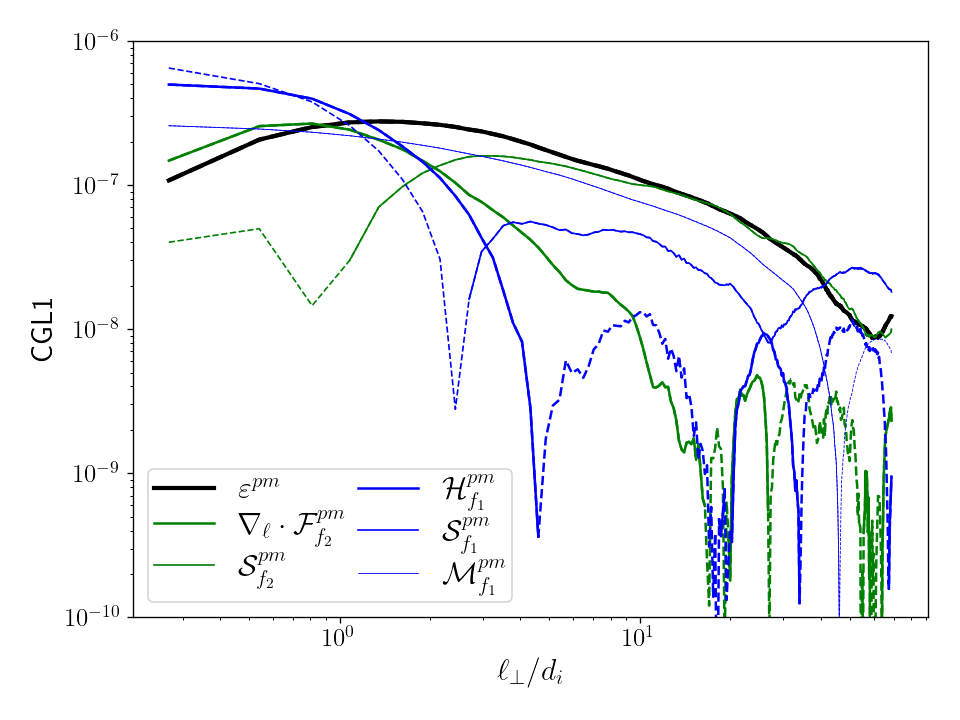
\includegraphics[width=0.49\linewidth,trim=1cm 1cm 1cm 1cm, clip=true]{./Mainmatter/Part_3/images_ch2/CGL1_f2pm_1D_lperp}
 \hfill
 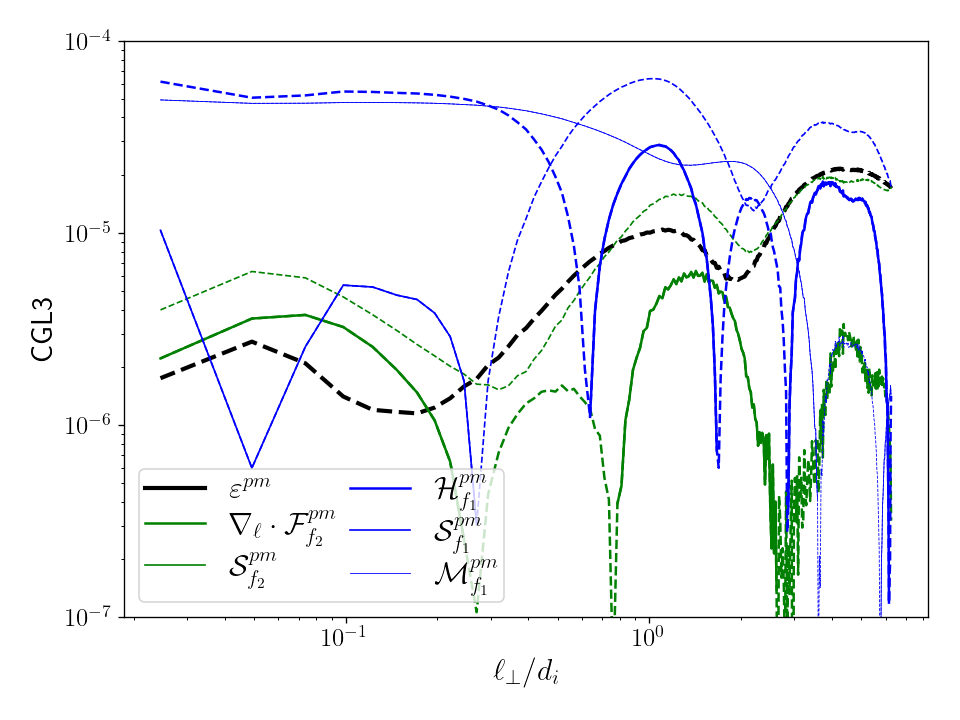
\includegraphics[width=0.49\linewidth,trim=1cm 1cm 1cm 1cm, clip=true]{./Mainmatter/Part_3/images_ch2/CGL3_f2pm_1D_lperp}
 \cprotect\caption{Panel d'étude de la reformulation de la contribution de pression magnétique \ensuremath{\varepsilon_{p}} (noir) dans CGL1 (gauche) et CGL3 (droite). \\ Bleu : Décomposition des termes de f1. Epais : contribution hybride \ensuremath{\mathcal{H}^{p}_{f_1}}. Moyen : contribution d'énergie magnétique \ensuremath{\mathcal{S}^{p}_{f_1}}. Fin :  contribution \ensuremath{\beta}-dépendante \ensuremath{\mathcal{M}^{p}_{f_1}}.\\Vert : Décomposition des termes de f2. Epais : terme flux \ensuremath{\nabla_{\boldsymbol{\ell}} \cdot \mathcal{F}^{p}_{f_2}}. Fin : termes sources \ensuremath{\mathcal{S}^{p}_{f_2}}. Représentation : 1D fonction de \ensuremath{\ell_{\perp}}.}
 \label{fig:elf2pm}
 \end{figure}
 
 Pour les deux simulations, la \figref{fig:elf2pm} montre que la décomposition (courbes bleues) en termes source, hybride et $\beta$-dépendant de la formulation f1 inspirée de \cacro{A18}, reflète moins bien la contribution de pression magnétique du taux de cascade que le découpage (courbes vertes) en termes flux et sources de f2. À l'exception de $\mathcal{S}^{pm}_{f_1}$ (dans le cas CGL1), ils sont loin de refléter individuellement $\varepsilon_{pm}$. A contrario,  $\mathcal{S}^{pm}_{f_2}$ reflète efficacement les variations et le signe de $\varepsilon_{pm}$ pour les deux simulations sauf pour les petites échelles de CGL1 où $\nabla_{\boldsymbol{\ell}} \cdot \mathcal{F}^{pm}_{f_2}$ domine. Notre décomposition semble donc plus adaptée pour la contribution de pression magnétique, cependant cela provient du caractère négligeable du nouveau terme flux (en général de l'ordre de $\SI{10}{\%}$ de $\varepsilon_{pm}$). 

 \paragraph{Reformulation des termes de pression entre f1 et f2 via \eqref{eq:turb_ref_p} :}
Une étude similaire peut être effectuée pour les termes composant $\varepsilon_{p}$ \eqref{eq:turb_ref_p}. 
 Ils seront découpés suivant : 
 \begin{itemize}
     \item f1 : la contribution hybride $\mathcal{H}^{p}_{f_1} = - \frac{1}{4} \nabla_{\boldsymbol{\ell}} \cdot \left<\left(1+\frac{\rho'}{\rho}\right) p \boldsymbol{v'} - \left(1+\frac{\rho}{\rho'}\right)p'\boldsymbol{v} \right>$
     \item f1 : la contribution de type source qui ne devient hybride que dans le cas isotherme, car $p/\rho$ est alors constant : 
         $\mathcal{S}^{p}_{f_1} =  \frac{1}{2} \left<\rho  \frac{p'}{\rho'} \nabla \cdot \boldsymbol{v'} + \rho' \frac{p}{\rho} \nabla \cdot \boldsymbol{v}\right>$
     \item f1 : la contribution qui peut être réécrite en appliquant le premier principe thermodynamique \eqref{eq:turb_ref_beta} $\mathcal{M}^{p}_{f_1} =  -\frac{1}{4} \left<\rho \frac{p'}{\rho'} \boldsymbol{v} \cdot \frac{\nabla'\rho'}{\rho'} + \rho' \frac{p}{\rho} \boldsymbol{v'} \cdot \frac{\nabla\rho}{\rho}  \right> $
     \item f2 : le terme flux $\nabla_{\boldsymbol{\ell}} \cdot \mathcal{F}^{p}_{f_2} = \frac{1}{4} \nabla_{\boldsymbol{\ell}} \cdot\left<\delta \rho  \delta \frac{p}{\rho} \delta \boldsymbol{v}\right> $ 
     \item f2 : les termes sources $\mathcal{S}^{pm}_{f_2} =  - \frac{1}{2}  \left<  \rho' \delta \left(\frac{p}{\rho}\right) \nabla \cdot \boldsymbol{v} -   \rho \delta \left(\frac{p}{\rho}\right) \nabla' \cdot \boldsymbol{v'} \right>\\-\frac{1}{4} \left<\left(\delta \rho \frac{p_*}{\rho} - \rho \delta \left(\frac{p}{\rho}\right)\right)\boldsymbol{v} \cdot \frac{\nabla' \rho'}{\rho'} - \left(\delta \rho \frac{p'}{\rho'} - \rho' \delta \left(\frac{p_*}{\rho}\right)\right)\boldsymbol{v'} \cdot \frac{\nabla \rho}{\rho}\right>$
 \end{itemize}
 \begin{figure}[!ht]
  \centering
  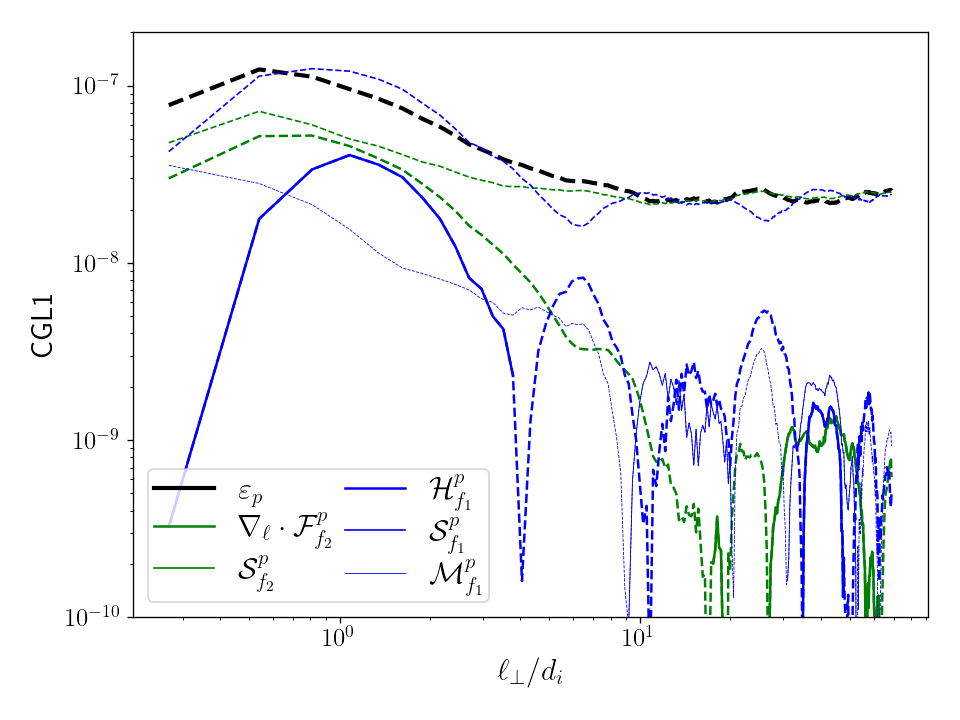
\includegraphics[width=0.49\linewidth,trim=1cm 1cm 1cm 1cm, clip=true]{./Mainmatter/Part_3/images_ch2/CGL1_f2p_1D_lperp}
 \hfill
 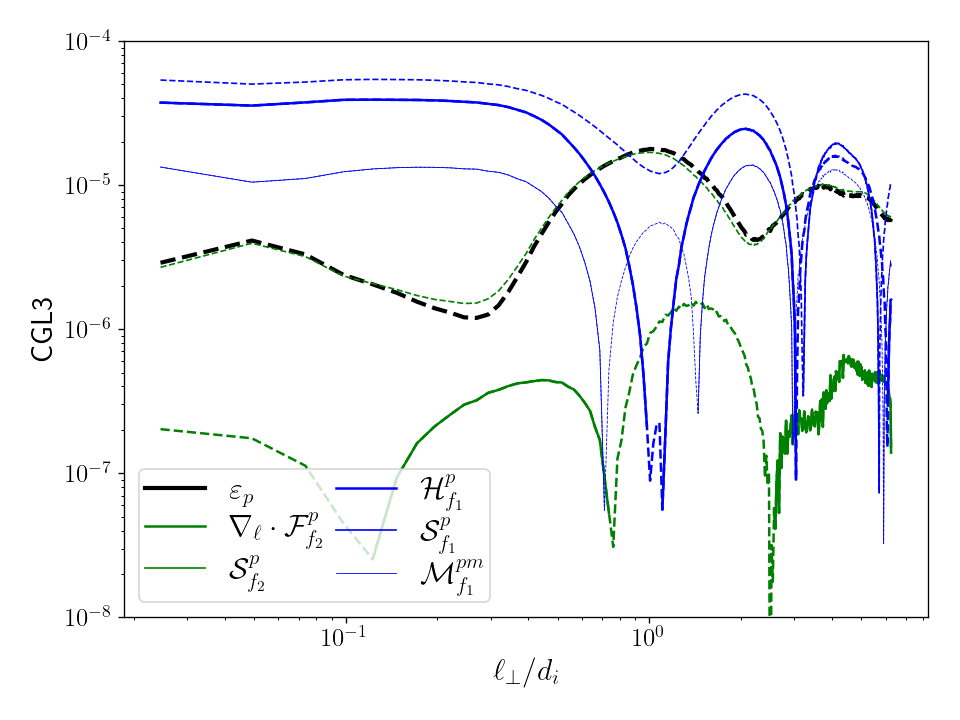
\includegraphics[width=0.49\linewidth,trim=1cm 1cm 1cm 1cm, clip=true]{./Mainmatter/Part_3/images_ch2/CGL3_f2p_1D_lperp}
 \cprotect\caption{Panel d'étude de la reformulation de la contribution de pression \ensuremath{\varepsilon_{p}} (noir) dans CGL1 (gauche) et CGL3 (droite). \\Bleu : Décomposition des termes de f1. Epais : contribution hybride \ensuremath{\mathcal{H}^{p}_{f_1}}. Moyen : contribution de type source qui ne devient hybride que dans le cas isotherme, \ensuremath{\mathcal{S}^{p}_{f_1}}. Fin : contribution qui peut être réécrite en appliquant le premier principe thermodynamique \ensuremath{\mathcal{M}^{p}_{f_1}}.\\Vert : Décomposition des termes de f2. Epais : terme flux \ensuremath{\nabla_{\boldsymbol{\ell}} \cdot \mathcal{F}^{p}_{f_2}}. Fin : termes sources \ensuremath{\mathcal{S}^{p}_{f_2}}. Représentation : 1D fonction de \ensuremath{\ell_{\perp}}.}
 \label{fig:elf2p}
 \end{figure}
 
 Les observations effectuées pour la contribution de pression magnétique au taux de cascade s'appliquent à la contribution de pression représentée sur la  \figref{fig:elf2p}. La formulation f2 séparant termes flux et termes sources semble plus appropriée pour représenter la cascade. Le terme flux $\nabla_{\boldsymbol{\ell}} \cdot \mathcal{F}^{p}_{f_2}$ est cependant un peu plus important dans la balance que ne l'est $\nabla_{\boldsymbol{\ell}} \cdot \mathcal{F}^{pm}_{f_2}$ dans le cas magnétique : autour de $\SI{30}{\%}$ de $\varepsilon_{p}$ pour CGL3 et complètement dominant aux petites échelles de CGL1. 
 
 Le comportement observé par \cacro{A18} reste donc valable dans nos simulations. Et avec les conclusions du Chapitre \ref{ch-14} et les résultats de cette section, on peut prédire que, pour l'application d'une formulation f2 dans des données faiblement compressibles, : 
 \begin{itemize}
     \item les termes flux de type Yaglom domineront les termes sources et les termes flux de pression, pression magnétique et énergie interne,
     \item la contribution des termes de flux de pression et pression magnétique sera négligeable devant celle des termes sources.
 \end{itemize}
 Le set de simulations \cacro{CGL} et \cacro{LF} n'étant pas adapté à une étude rigoureuse du caractère systématique de la validité de ces prédictions ni à une analyse de l'évolution de ces contributions en fonction de la compression du milieu telle que celle effectuée par \cacro{A18}, ces résultats resteront sous la forme de résultats préliminaires. Je me suis aussi posée la question de l'apport de la formulation f3 sur la formulation f2 via \eqref{eq:turb_ref_ptot}. Les résultats, non présentés ici, ne semblent montrer aucun apport significatif.
 
 En interprétant les termes flux en tant qu'énergie transférée à travers les échelles et les termes sources tels des réservoirs d'énergie localisés aux différentes échelles, il semble ici que les contributions de pression magnétique et thermodynamique aient plutôt des rôles de réservoirs. L'augmentation des termes flux aux petites échelles de CGL1 indiquerait, avec cette interprétation, le lieu d'un transfert d'énergie à travers les échelles permis par ces pressions\footnote{Il serait intéressant de démontrer analytiquement ces comportements à l'aide d'une théorie plus locale telle que la théorie du \og coarse-graining \fg{} qui a permis de démontrer l'existence d'une cascade d'entropie par exemple [\cite{eyink_cascades_2018}]}.
% 
% %%%%%%%%%%%%%%%%%%%%%%%%%%%%%%%%%%%%%%%%%%%%%%%%%%%
% % \paragraph{Reformulation des termes de pressions totales entre f2 et f3 via \eqref{eq:turb_ref_ptot} :}
% % Dans la formulation f3, la contribution de pression totale, $\varepsilon^{p_*}$, est reformulée (voir \eqref{eq:turb_ref_ptot}). Afin de déterminer l'apport de f3 par rapport à f2, sont définies les quantités suivantes : 
% % \begin{itemize}
% %     \item f2 : le terme flux $\nabla_{\boldsymbol{\ell}} \cdot \mathcal{F}^{p_*}_{f_2} = \frac{1}{4} \nabla_{\boldsymbol{\ell}} \cdot\left<\delta \rho  \delta \frac{p}{\rho} \delta \boldsymbol{v}\right> $ 
% %     \item f2 : les termes sources $\mathcal{S}^{p_*}_{f_2} = - \frac{1}{4} \left<\left(\delta \rho \frac{p_*}{\rho} - \rho \delta \left(\frac{p_*}{\rho}\right)\right)\boldsymbol{v} \cdot \frac{\nabla' \rho'}{\rho'} - \left(\delta \rho \frac{p'_*}{\rho'} - \rho' \delta \left(\frac{p_*}{\rho}\right)\right)\boldsymbol{v'} \cdot \frac{\nabla \rho}{\rho}\right>$
% %     \item f3 : le terme flux $\nabla_{\boldsymbol{\ell}} \cdot \mathcal{F}^{p_*}_{f_3} = - \frac{1}{4} \nabla_{\boldsymbol{\ell}} \cdot\left<\delta p_*  \delta \left(1/\rho\right) \delta\left(\rho \boldsymbol{v}\right)\right> $ 
% %     \item f3 : les termes sources $\mathcal{S}^{p_*}_{f_3} = - \frac{1}{4}\left< \delta \left(p_*\right) \rho \boldsymbol{v} \cdot \nabla'\left(\frac{1}{\rho'}\right) - \delta \left(p_*\right) \rho' \boldsymbol{v'} \cdot \nabla \left(\frac{1}{\rho}\right)\right>$ 
% % \end{itemize}
% % \begin{figure}[!ht]
% %  \centering
% % 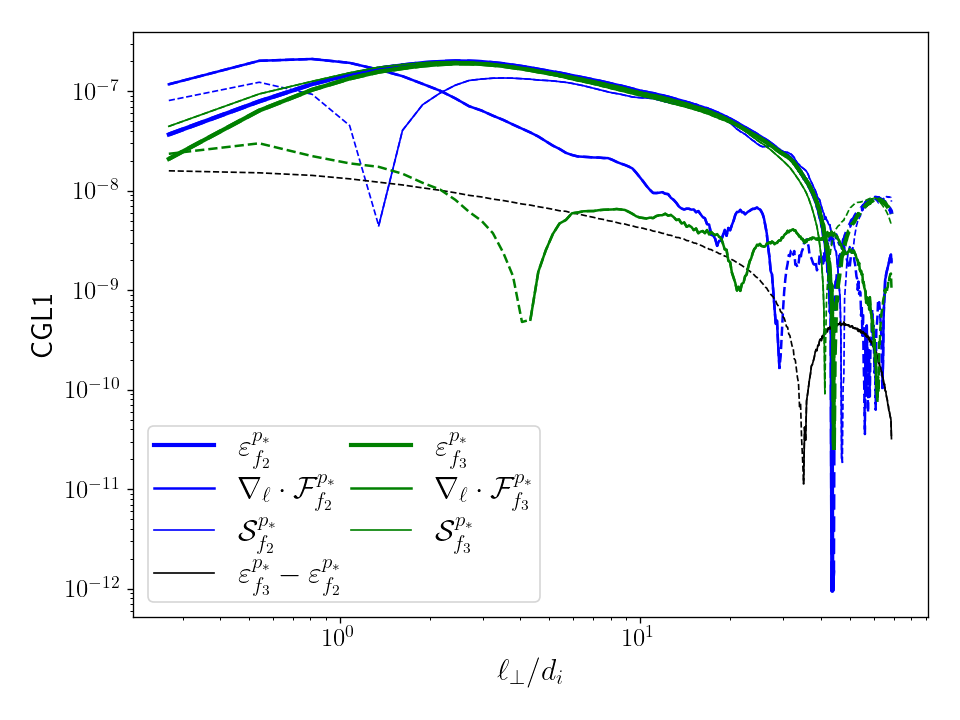
\includegraphics[width=0.49\linewidth,trim=1cm 1cm 1cm 1cm, clip=true]{./Part_3/images_ch2/CGL1_f3_1D_lperp}
% % \hfill
% % 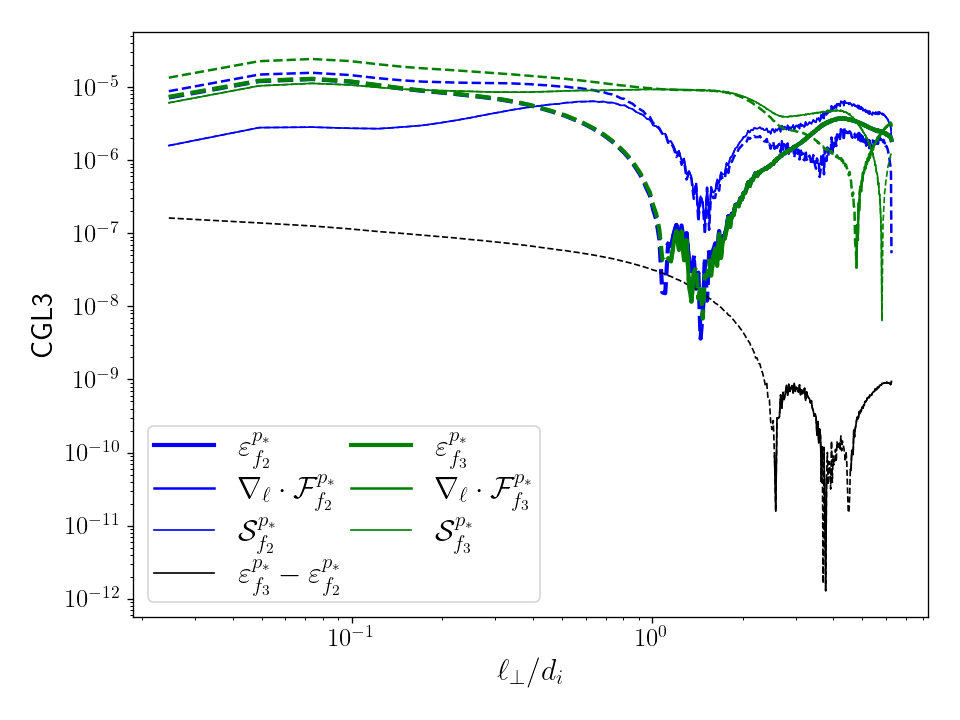
\includegraphics[width=0.49\linewidth,trim=1cm 1cm 1cm 1cm, clip=true]{./Part_3/images_ch2/CGL3_f3_1D_lperp}
% % \cprotect\caption{Détails des termes flux (épaisseur moyenne) et sources (épaisseur fine) de $\varepsilon^{p_*}$ (épaisseur épaisse) obtenu via les formulations f2 (bleu) et f3 (vert). La différence  $\varepsilon^{p_*}_{f_3}-\varepsilon^{p_*}_{f_2}$ correspond à la courbe noire. Représentation : 1D fonction de $\ell_{\perp}$. Gauche : CGL1. Droite : CGL3}
% % \label{fig:elf3}
% % \end{figure}
% 
% % La figure \figref{fig:elf3} montre une répartition différente entre f2 et f3 de la contribution de pression totale sur les termes flux et sources. La différence entre la contribution écrite via f2 et celle écrite via f3 (courbe noir) n'est pas de l'ordre du zéro numérique, contrairement aux résultats sur la reformulation entre f2 et f1. On suspecte une erreur dans l'implémentation des termes de f3, mais cette dernière n'a pas été identifiée. Par la suite, on n'utilisera donc pas f3.  


\chapter{Details du terme correctif anisotrope pour CGL3B, CGL5 et CGL6}\label{an:Pi}
        \renewcommand\partie{\Partie\ Annexe \thechapter}
        
 \begin{figure}[!ht]
  \centering
  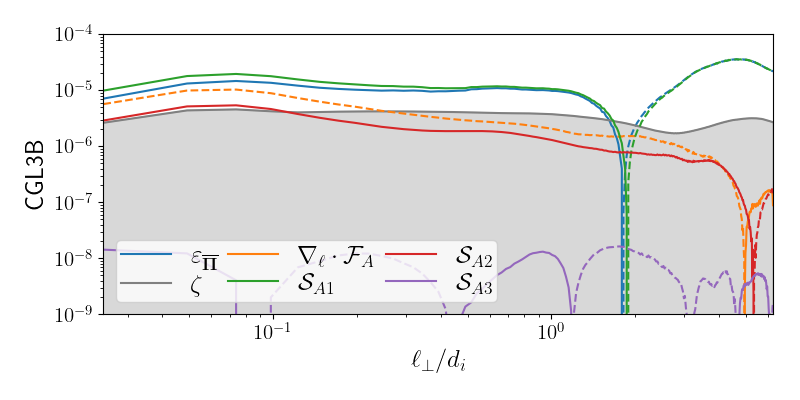
\includegraphics[width=0.8\linewidth,trim=0cm 1.3cm 0cm 0.5cm, clip=true]{./Mainmatter/Part_3/images_ch3/CGL3B_compa_cgl}
 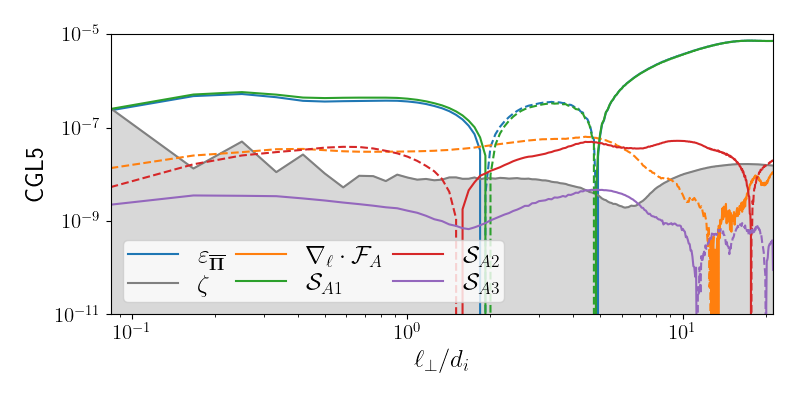
\includegraphics[width=0.8\linewidth,trim=0cm 1.3cm 0cm 0.5cm, clip=true]{./Mainmatter/Part_3/images_ch3/CGL5_compa_cgl}
  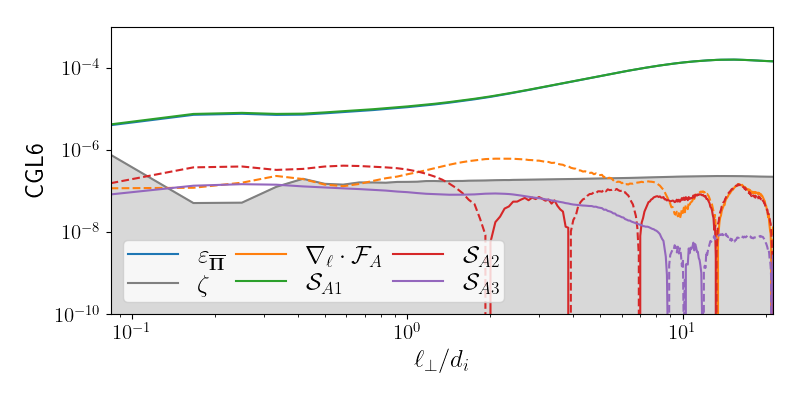
\includegraphics[width=0.8\linewidth,trim=0cm 0.5cm 0cm 0.5cm, clip=true]{./Mainmatter/Part_3/images_ch3/CGL6_compa_cgl}
 \cprotect\caption{Simu : CGL3B (haut), CGL5 (milieu) et  CGL6 (bas). Représentation \cacro{1D} en fonction de \ensuremath{\ell_{\perp}} du détail de \ensuremath{\varepsilon_{\overline{\boldsymbol{\Pi}}}} (bleu). Orange : \ensuremath{\nabla_{\boldsymbol{\ell}} \cdot \boldsymbol{\mathcal{F}_A}}. Vert : \ensuremath{\mathcal{S}_{A1}}. Rouge : \ensuremath{\mathcal{S}_{A2}}. Violet : \ensuremath{\mathcal{S}_{A3}}. Gris : niveau d'erreur \ensuremath{\zeta}. Les termes présents dans la zone grise délimitée par \ensuremath{\zeta} sont supposés négligeables. }
 \label{fig:detail_pi_CGL3B-5-6}
 \end{figure}
